%!TEX program = pdflatex
\documentclass[conference,10pt,a4paper]{IEEEtran}

\usepackage[utf8]{inputenc}
\usepackage[T1]{fontenc}
\usepackage[american]{babel}

\usepackage[acronym, nomain, nowarn]{glossaries}
\loadglsentries{acronyms}
\usepackage{csquotes}
\usepackage{booktabs}

\usepackage{url}

\usepackage{amssymb}
\usepackage{mathtools}
\usepackage{fixmath}
\usepackage{algorithm2e}
\usepackage{subcaption}

\usepackage{eurosym}
\usepackage{siunitx}
\sisetup{load-configurations = abbreviations,
         binary-units, 
         per-mode=symbol, 
         detect-weight=true, 
         detect-family=true}
\DeclareSIUnit{\EUR}{\text{\euro}}

\usepackage[url=false,
            doi=true,
            backend=biber,
            style=ieee,
            isbn=false,
            sorting=none]{biblatex}
\addbibresource{literature.bib}

\usepackage{tabu}
\makeglossaries

\usepackage[inline]{enumitem}

\usepackage[np]{numprint}
\usepackage{balance}

\npstyleenglish


\begin{document}

\title{Crowdsensed QoE for the Community}



\author{\IEEEauthorblockN{Florian Metzger}
\IEEEauthorblockA{
Chair of Communication Networks\\
University of Würzburg, Germany\\
%Essen, Germany\\
florian.metzger@uni-wuerzburg.de}
\and
\IEEEauthorblockN{Tobias Hoßfeld}
\IEEEauthorblockA{
Chair of Communication Networks\\
University of Würzburg, Germany\\
%Essen, Germany\\
tobias.hossfeld@uni-wuerzburg.de}}

\maketitle

%!TEX root = paper.tex
%%%%%%%%%%%%%%%%%%%%%%%%%%%%%%%%%%%%%%%%%%%%%%%%%%%%%%%%%%%%%%%%%%%%%%%%%%%%%%%%
\begin{abstract}

In recent years several community testbeds as well as participatory sensing  platforms have successfully established themselves to provide open data to everyone interested. Each of them with a specific goal in mind, ranging from collecting radio coverage data up to environmental and radiation data. Such data can be used by the community in their decision making, whether to subscribe to a specific mobile phone service that provides good coverage in an area or in finding a sunny and warm region for the summer holidays.

However, the existing platforms are usually limiting themselves to directly measurable network \acrshort{QoS}. If such a crowdsourced data set would provide more in-depth derived measures, this would enable an even better decision making. A community-driven crowdsensing platform that derives spatial application-layer user experience from resource-friendly bandwidth estimates would be such a case, video streaming services come to mind as a prime example. In this paper we present a concept for such a system based on an initial prototype that eases the collection of data necessary to determine mobile-specific \acrshort{QoE} at large scale. In addition we reason why the simple quality metric proposed here can hold its own.
\end{abstract}

%!TEX root = paper.tex
%%%%%%%%%%%%%%%%%%%%%%%%%%%%%%%%%%%%%%%%%%%%%%%%%%%%%%%%%%%%%%%%%%%%%%%%%%%%%%%%
\section*{Preface}


\textit{This paper was originally written in 2017, but never published. We think, the idea to engage the community in crowdsensing with easy-to-understand and practical information without burdening them has even increased in merit today, and we strife to continue this work in the future.} 

\textit{Therefore, we wanted to preserve this work in the form it was originally prepared in 2017, with updated affiliations, restored links, and this preface. Past reviewers of this manuscript mostly criticized the small scale of this study and the lack of details and evaluation with regards to the bandwidth estimation, the QoE model, and the geographical visualization. Reviewers praised the dissemination of easily interpretable information from science to citizens using a decentralized approach.}
%!TEX root = paper.tex
%%%%%%%%%%%%%%%%%%%%%%%%%%%%%%%%%%%%%%%%%%%%%%%%%%%%%%%%%%%%%%%%%%%%%%%%%%%%%%%%
\section{Introduction}
\label{sec:introduction}

Be honest: Did you ever try using your flavor-of-the-month messaging or
social app and just couldn't get it to work? Despite all information
available to you claiming otherwise. Or did you want to watch a stream
but only received a video in abysmal quality despite having an excellent
connection?

An example: One of the author's routinely commutes to work by tram.
While waiting at the underground tram station he tends to read his
Twitter stream. In about 50\% of cases the author's device does not
receive any data despite a full signal strength and data indicator. Only
after putting a significant distance between himself and the station the
data transmission resumes.

If this is the case then you are in the same boat as the authors. and
many other people. And lo and behold! This situation can be improved
upon, continue reading to find out how.

We --- as in we, the research community --- have reached a point where we have a rather good understanding of video streaming \gls{QoE}. Many a user study has been conducted to ascertain the subjective aspects of video quality, both in lab environments as well as through crowdsourcing. From the results of these, application layer \gls{QoS} and \gls{QoE} models have been derived that affix some quality rating to certain objectively measurable \gls{QoS} metrics. This begs the question: What does one actually do with this information? How can it be used to one's benefit? One such benefit will be the contribution of this paper in the form of a mapping service displaying service-specific quality information derived from community-driven network measurements.

In the past video streaming \gls{QoE} research was often incentivised by both video streaming service providers and home Internet access providers. The former obviously desired to understand how their service is received and thus improved their system based upon this information. The latter entities aspire to understand the traffic composition flowing through their network and the resulting direct implications on their customers, not in terms of easy-measurable-but-hard-to-interpret network \gls{QoS} metrics but rather as direct customer satisfaction, e.g. \gls{QoE} measures.

However, there is another, third, party that has seen not much direct benefit from these endeavors: the actual consumers of video streams. Currently, if a user watches a video she can typically only assess her own subjective video quality herself. The results from user studies and \gls{QoE} models are mostly not readily available to be applied to home users directly. And this situation becomes even more interesting when looking at mobile users, where one often desires to know if one's mobile device works at a specific location. But these current mobile network conditions are very location-dependent and might fluctuate based on a great many factors. This includes spatio-temporal properties, but also radio propagation effects as well as mobility issues and the other usual kinks of a shared medium (as the multiplexed resource allocation in today's mobile radio technologies provides).

Now take a look at the recent developments around mobile crowdsourcing, participatory crowdsensing and community-run testbeds and data-collection programs. You can partake in projects like radio coverage collection\footnote{E.g. \url{https://opensignal.com/}, \url{https://radiocells.org/}, and \cite{raf2013sensorium}.}, current weather information\footnote{E.g. \url{https://web.archive.org/web/20170703191919/http://weathersignal.com/about/}.}, air quality data\footnote{E.g. \url{http://airqualityegg.com/}.}, community-run Internet access\footnote{E.g. the German Freifunk project.}, or even environmental radiation monitoring\footnote{E.g. \url{https://safecast.org/}.} with little to no effort, using either one's own mobile phone or, alternatively, affordable sensor boards. Such projects flourish both through the immediate benefits one can gain through the available data and the participatory motif.

However, most of these community-driven efforts concern basic, directly measurable data. Only very rarely \cite{Nam:2014:YPA:2619239.2631433,7194076} have application-layer \gls{QoS} and \gls{QoE} models and mappings been applied to such data for an immediate benefit of the participants. Exploring the opportunities of this crossover is the goal of this work. Specifically, for this paper we want to tackle the question of YouTube's streaming quality on-the-go on the basis of location-specific bandwidth estimates collected from participating mobile devices.

In order to do so, after highlighting all the related and similar projects as well as the necessary research foundations in Section~\ref{sec:relatedwork}, we describe a mobile crowdsensing prototype --- aimed at low resource usage to have a negligible performance impact in order to be scalable --- that collects the network \gls{QoS} data required for input to an appropriate \gls{QoE} mapping in Section~\ref{sec:prototype}. In the following Section~\ref{sec:qoe} the collected data is fed into a simple, but effective \gls{QoE} mapping and the results evaluated. We further discuss potential approaches how these quality ratings can be appropriately visualized, especially with geospatial and other context data in mind. The work is concluded in Section~\ref{sec:conclusion}.

%!TEX root = paper.tex
%%%%%%%%%%%%%%%%%%%%%%%%%%%%%%%%%%%%%%%%%%%%%%%%%%%%%%%%%%%%%%%%%%%%%%%%%%%%%%%%
\section{Related Work and Background}
\label{sec:relatedwork}

In order for such an approach to succeed quite a few different lines of work need to be reconciled here. Namely:
\begin{itemize}
	\item Crowdsourcing and participatory sensing methods,
	\item the intricacies of community networks and testbeds,
	\item subjective video streaming user studies,
	\item Resource-friendly network \gls{QoS} measurements
	\item the relationship of network \gls{QoS} to video \gls{QoE} and mappings thereof.
\end{itemize}

Each of these individual sectors and work essential for this QoE-crowdsensing approach are briefly covered in this section.


%%%%%%%%%%%%%%
\subsection{Crowdsourcing, Crowdsensing and Experiences with Existing Community Campaigns}

Targeting a participatory crowdsourcing approach for large-scale \gls{QoE}-mappings is a challenging endeavor, therefore building on past experiences and best practices is crucial. For example, crowdsourced network measurements raise the issue of trust in the collected data, as it could have been, willingly or unwillingly, falsified \cite{Tanas2014,Hirth201585}. This needs to be dealt with the proper verification and statistical methods.

The concept of participatory sensing (e.g. \cite{Dutta:2009:CSP:1644038.1644095,Shilton:2009:FBL:1592761.1592778}) has now been around for a few years and quite a number of projects exist now that aim to gather and make available sensed data to the community, e.g. air quality data in \cite{partisensing2006} or vehicular traffic~\cite{Herrera2010568}. %, or public transportation incidents in \cite{Tanas2013}.
Campaigns that aim to put a data-collecting application unto one's mobile phone have to deal with significant privacy concerns, as they usually not only have access to the devices current location but also to all communication, sensor readings and files stored on the device. One of the ways to resolve this is to give the user fine-grained control over the data to be used in the campaign, and also ensure its secure and anonymized transmission \cite{raf2013sensorium,albert2016mess,zhuang2015login}.


%%%%%%%%%%%%%%
\subsection{Resource-Friendliness and Mobile QoS-Measurements}

In order to encourage a wide-spread proliferation of the campaign --- an absolute must when dealing with location-specific cellular measurement data --- the data-collecting mobile phone application should adhere to stringent resource-restrictions. This would enable an installation on a wider selection of devices as well as allows it to run in the background without interfering with other daily activities of the participants. This especially concerns both the battery life as well as the used radio resources (which in turn generates high energy usage as well) and traffic data caps. To tackle the latter, direct throughput measurements need to be avoided. Instead, various bandwidth estimation methods come to mind that attempt to compute the actual currently possible throughput through specific transmission side effects --- like the inter-arrival time of two consecutively sent \acrshort{TCP} segments in the Packet Pair method \cite{Lai01nettimer:a,Ribeiro:2004:SAB:1005686.1005734,Strauss:2003:MSA:948205.948211}. This works quite well in stable wired networks, but can have issues in radio networks (cf. also \cite{6918916} and Section~\ref{sec:BWest}). Concerning energy consumption, \cite{schwartz13angryapps,6664206} gives some pointers as to the root causes of these in relation to smartphone applications.

%%%%%%%%%%%%%%
\subsection{Subjective Studies on Video Streaming Quality and Quality Models}

After the network \gls{QoS} data has been collected it needs to be transformed to the desired target \gls{QoE} metric. The goal in this work was to project YouTube streaming quality. So, for an adequate mapping of measured transmission characteristics to be defined, first the service's properties have to be fully understood and described. Thankfully, many prior publications on YouTube's adaptive streaming mechanisms readily exist, e.g. \cite{7810251,7497231}. Indeed, many interactive YouTube subjective quality user studies have been conducted in the past \cite{7194076,Nam:2014:YPA:2619239.2631433}, and guidelines to conduct further crowdsourced subjective video quality studies also exist \cite{7148150}. And they all paint a good picture of YouTube's streaming experience. However, they are hard to scale up to much more participants, due to the time and resource investments required by the users, amongst other reasons. Of special interest to this work are studies that link the user experience to bandwidth as is for example done in \cite{Casas:2015:EQC:2785971.2785978}. This study finds, that \SI{4}{\mega\bit\per\second} produce a near-optimal experience in their scenario. Yet other studies (e.g. \cite{7247426}) suggest that it is not the value of throughput itself that is decisive, but instead the throughput variations that have a large impact on the user experience. However, other work also suggests that the correlation of throughput could actually be almost neglible \cite{7562672}. Indeed, many other operational factors and also especially anomalies can have a large impact on the \gls{QoE} (as e.g. shown in the case of YouTube in \cite{6975242}).

To achieve independence of this interactive user component, models that appropriately map network \gls{QoS} to an application layer representation of quality are necessary. While there are models for non-adaptive streaming that map the number and length of stalling events to a \gls{MOS} value \cite{Hossfeld2013}, research on good adaptive streaming quality models has not yet progressed very far. However, works exist that discuss \gls{QoE} modeling for video streaming in general \cite{7148138}. A further survey \cite{6913491} describes the intricacies of \gls{HAS} that are necessary to understand in order to appropriately conduct \gls{QoE} modeling. For the purposes of the work in this manuscript we aim for a simple available-throughput-to-achievable-video-quality mapping. On this matter it is also interesting to find \textit{acceptable} levels of \gls{QoE}, or specifically of \gls{MOS}, to a user group in order to link this level to metrics that a user of a participatory crowdsensing platform can easily understand.

For a mobile \gls{QoE}-crowdsensing campaign it is not only beneficial to conduct regular, location-based network \gls{QoS} measurements, but also to couple this with further context data, i.e. device information and sensor readings. The importance of such \textit{context factors} in \gls{QoE} monitoring has been discussed in, e.g., \cite{7140480}. In this specific case context information can be used to accurately handle the ``tunnel scenario'' \cite{7511206,Metzger2016246} to provide even better quality predictions to the community in the future.
%!TEX root = paper.tex
%%%%%%%%%%%%%%%%%%%%%%%%%%%%%%%%%%%%%%%%%%%%%%%%%%%%%%%%%%%%%%%%%%%%%%%%%%%%%%%%
\section{The Crowdsensing Mobile App Prototype}
\label{sec:prototype}

A community crowdsensing service faces several challenges in its task of gathering and processing the data before making it available in a concise and easy-to-understand visualized way. The goal for the gathering portion is to measure in an automated, non-interactive fashion in order to be non-intrusive to the participants as well as reach a larger audience. This allows for a larger geographical coverage of the project service quality values while simultaneously being more conservative with the available resources. The implementation of these aspects is discussed in this section.


%%%%%%%%%%%%%%%%%%%%%%%%%%%%%%%%%%%%%%%%%%%%%%%%%%%%%%%%%%%%%%%%%%%%%%%%%%%%%%%%
\subsection{The Issue of Bandwidth Measurements}
\label{sec:BWest}

The most important directly measurable network \gls{QoS} metric for a \acrshort{TCP}-based video streaming service is arguably the achievable goodput of this flow. Typically, this would be calculated by downloading a file from a remote location and dividing its size by the time it took to transmit it. This is inherently an average value over a certain time period, which makes it tricky to pinpoint it to specific spatial coordinates when this is employed during a mobile crowdsensing campaign.

Furthermore, it is especially crucial to not waste the participants monthly data caps solely on the estimation of video streaming quality. In some countries the monthly contractual data caps are set extremely low. For example, in Germany postpaid contracts with a data cap of \SI{1}{\giga\byte} currently cost a monthly fee of around \SI{25}{\EUR}. On the other hand, only measuring the user's actually watched video streams would provide an insufficient amount of samples for providing accurate data for mobile networks. This means that in order to widen the possible audience, direct throughput measurements of streaming services are out of the question. Our measurement prototype attempts to solve these issues by implementing several bandwidth estimation methods, which trade a loss of accuracy for much less data and time usage. The rest of this section aims to evaluate if the precision of these methods is sufficient for the \gls{QoE} crowdsensing endeavor.


\subsubsection{Bandwidth Estimation Methods: Basics and Variants}

These bandwidth estimators can be roughly divided into two different categories. Approaches from the first category, namely \textit{Cross-Traffic Estimation}, actively send a small amount of probe packets with fixed inter-packet times. On the bottleneck link the timing of these are altered through network throughput limitations as well as traffic from other sources, from which the bandwidth can then be calculated. One well-known representative of this category is Packet Pair~\cite{Bolot:1993:EPD:167954.166265,749288}. The second set of approaches, termed \textit{Self-Induced Congestion}, relies also on active probes, but here they are meant to briefly congest the network themselves in order to observe the resulting path characteristics. Packet Train~\cite{Jain02pathload:a} is one such variant implemented here.

It should be noted that some methods require the presence of an actively sending server under the control of the measurement client with the possible benefit of a better measurement accuracy, making it unfeasible to measure public services like YouTube with them. Packet Pair is one of them. However, it is also usually possible to circumvent this requirement by exploiting known properties of \acrshort{TCP}. For example, some approaches \cite{saroiu2002sprobe,Chakravarty08linkwidth:a} force the transmission of \gls{TCP} RST packets through specifically crafted \gls{TCP} SYN packets and then time the interaction.


%%%%%%%%%%%%%%%%%%%%%%%%%%%%%%%%%%%%%%%%%%%%%%%%%%%%%%%%%%%%%%%%%%%%%%%%%%%%%%%%
\subsection{Prototype and Estimator Evaluation}

To evaluate the feasibility of these methods as well as to establish a foundation for the participatory crowdsensing aspects a prototype was set up. This was realized as a Java-based Android application. Both the prototype, with the bandwidth estimation and data collection and upload methods\footnote{\url{https://github.com/mas-ude/bw-estimation-App}}, and the  server-side components required for some of the bandwidth estimation methods\footnote{\url{https://github.com/Nobodi/Bandwith-Estimation}}, are available online.

\begin{figure}[!t]
	\centering
	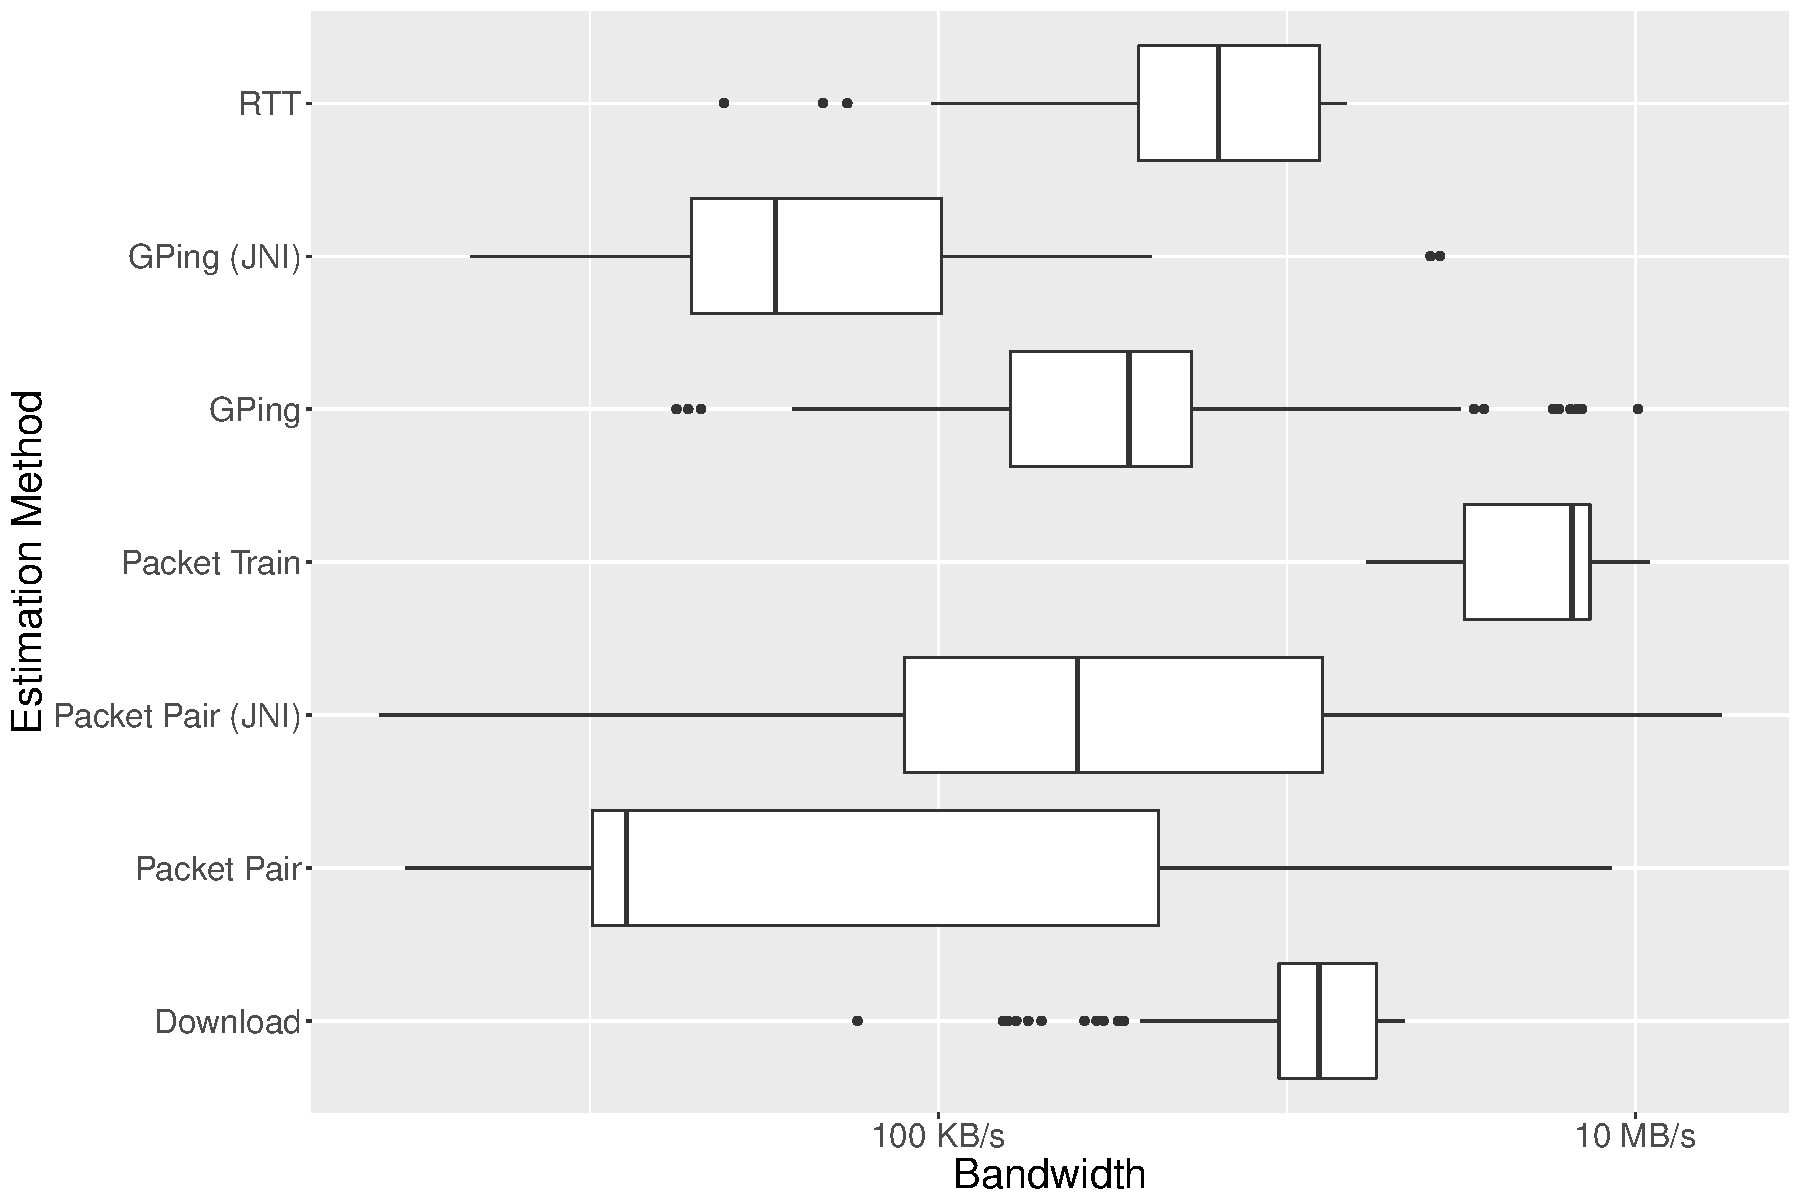
\includegraphics[width = 1.0\columnwidth]{images/BWest-boxplots.pdf}
	\caption{Boxplots of the various tested throughput estimation methods in the evaluation scenario. Entries denoted with JNI use system-level packet and timing facilities in an attempt to improve accuracy.}
\label{fig:boxplots}
\end{figure}

Evaluating the addressed estimation methods is not as straight-forward as one might expect in a mobile environment due to the many factors that can influence the results to a small or large degree. To compensate for these factors this evaluation was conducted in a more controlled setting. All evaluations ran on a single mobile phone, an \textit{LG G3}, and were fixed to a single location to avoid varying radio conditions. Similarly, all corresponding runs were closely grouped together to ensure reasonable temporal coupling. These runs were conducted in five-minute intervals for roughly one day. Various methods described in the literature (as mentioned above) were tested in comparison to the results from simple download tests with a large file. The method dubbed `RTT' is a variant of download, but is using very small files, transferred from a controlled server environment, to calculate its throughput estimate, making it potentially less accurate.

\begin{table}[!t]
\caption{Data usage of the estimation methods.}
\label{tab:datausage}
	\begin{tabu}{XSS}
		\toprule
		 & {\textbf{Used Volume (\si{\kilo\byte})}} & {\textbf{Duration (\si{\second})}} \\
		 \midrule
		\textbf{Download} & 10240 & 9.42 \\
		\textbf{RTT} & 256 & 0.36 \\
		\textbf{Packet Pair} & 6 & 0.37 \\
		\textbf{GPing} & 2.5 & 0.14 \\
		\textbf{Packet Train} & 437 & 0.89 \\ % 437 -- 6035 
		\bottomrule
	\end{tabu}
\end{table}

Figure~\ref{fig:boxplots} depicts the results attained from this scenario. The inter-quartile ranges of the accumulated samples reveal, with every method except RTT, rather large deviations from the download results. The root cause is unclear in this limited evaluation, but this kind of estimation error does not come entirely unexpected due to the aforementioned temporal instability of mobile networks, even in a static location. All of the applied methods generally expect certain network properties to hold that are unfortunately only loosely applicable to mobile networks, with their strong form of a signaling plane. On approach to remedy this situation is to apply an adjustment factor to the individual methods if the offset to the download results proves to be stable enough in a wider range of scenarios.

However, one other benefit is clear when looking at the data and time used during the measurements in Table~\ref{tab:datausage}. The intended goal of being more resource-friendly in order to target a wider audience can be easily fulfilled with these methods, especially with the single-pair approaches Packet Pair and GPing, allowing for more frequent probing and thus more coverage on a crowdsensed community \gls{QoE} map.

%!TEX root = paper.tex
%%%%%%%%%%%%%%%%%%%%%%%%%%%%%%%%%%%%%%%%%%%%%%%%%%%%%%%%%%%%%%%%%%%%%%%%%%%%%%%%
\section{Quality Model, Mappings and Map}
\label{sec:qoe}

Speaking of community maps, this bring us to the final tasks of interpreting the collected data as YouTube quality and presenting it in an easy-to-grasp way to the community. As discussed in Section~\ref{sec:relatedwork} there do exists metrics that derive a higher layer abstraction from directly measurable values, such as the bitrate. E.g. \cite{hossfeld2011transport} fitted the \textbf{stalling frequency} $F$ from throughput samples as

\begin{equation*}
F(X) = -1.09 e^{-1.18 \frac{V}{B}} + 0.36
\end{equation*}

for transmission bandwidths $B$ and video bitrates $V$. But a stalling frequency is nothing that can be easily understood in terms of YouTube quality by the community, and therefore a simpler metric is desired. For this let's consider the \textbf{reception rate} $\rho = \frac{B}{V}$ \cite{Hossfeld2013}. This means that as long as the transmission rate is above the video rate the video streaming should work well, bar any variations. This is even more so if you include a safety margin as evaluated in, e.g., \cite{Zinner2015}. A \SI{25}{\percent} surplus of the transmission rate should therefore take care of this and ensure the video to be playable at the selected quality level at all times. This then yields a definition of the playable video quality $v_{playable}$ for our system as

\begin{equation*}
\phantom{\text{.}} v_{playable} = \max\left(\left\{ v | v \in \mathbb{V} \wedge 1.25 \cdot v < B \right\}\right) \text{.}
\end{equation*}

Used as the set of $V$ is here simply YouTube's recommended video encoding bitrates\footnote{Based on information from \url{https://support.google.com/youtube/answer/1722171?hl=en}. Do note that these are recommendations for the video upload before they are transcoded by YouTube. But this gives a rough estimate for the download bitrate as well.} as listed in Table~\ref{tab:recvidbr}.

\begin{table}[!t]
	\caption{Recommended YouTube video bitrates for 30 fps video, mean stalling frequency, and ratio of bandwidth samples above $1.25 \times V$ in the measurement data.}
	\label{tab:recvidbr}
	\begin{tabu}{XSSS}
	\toprule
	\textbf{Res.} & {\textbf{Video Bitrate}} & {\textbf{Stalling Frequency}} & {\textbf{Ratio of} $\mathbf{B}$} \\
	& {$\mathbf{V}$ (\textbf{\si{\mega\bit\per\second})}} & $\mathbf{F}$ & {\textbf{above} $\mathbf{1.25 \times V}$} \\
	\midrule
	\textbf{2160p} & 45 & 0.35 & 0 \\
	\textbf{1440p} & 16 & 0.23 & 0 \\
	\textbf{1080p} & 8 & 0.09 & 0.34 \\
	\textbf{720p} & 5 & 0.04 & 0.67 \\
	\textbf{480p} & 2.5 & 0.01 & 0.90 \\
	\textbf{360p} & 1 & 0.00 & 0.98 \\
	\bottomrule
	\end{tabu}
\end{table}

\begin{figure}[!t]
    \centering
    \begin{subfigure}[b]{0.45\columnwidth}
        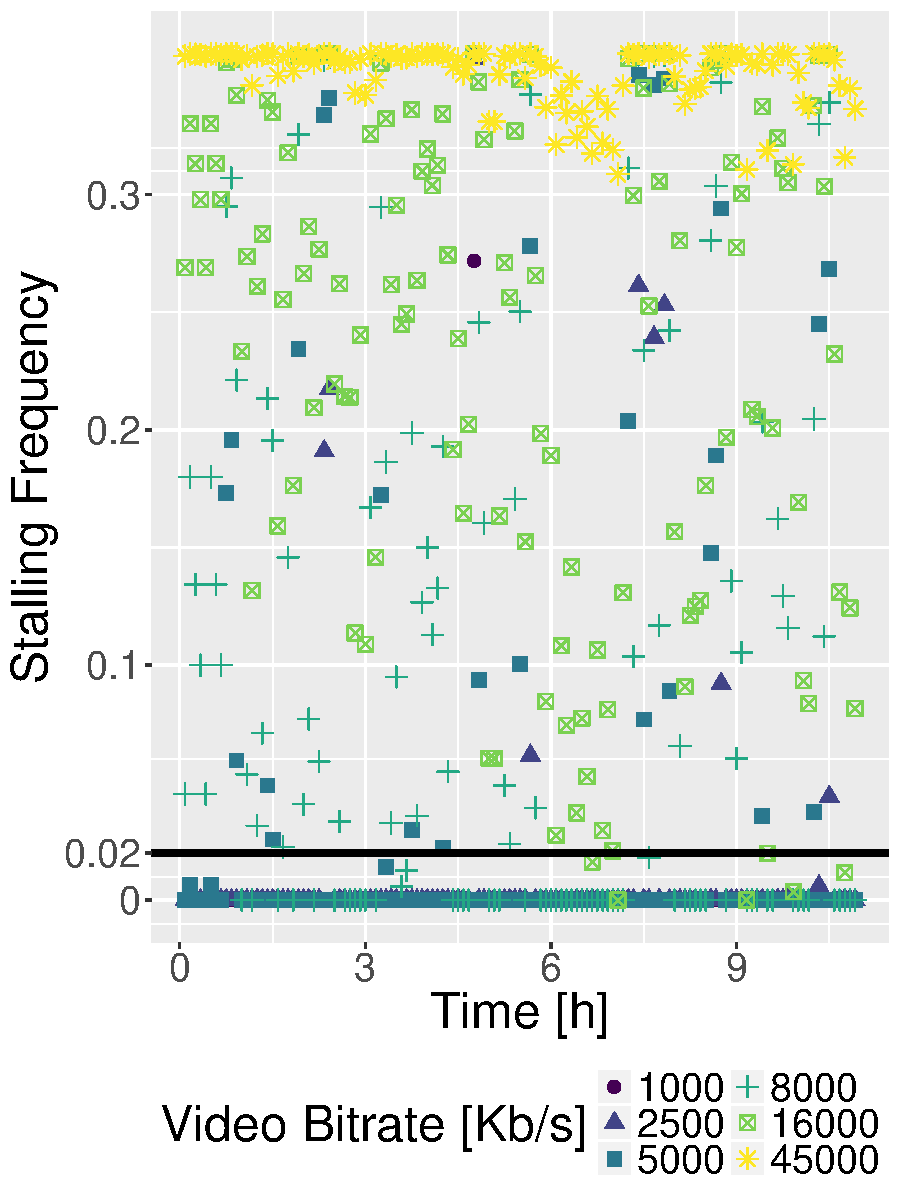
\includegraphics[width=\textwidth]{images/stallingfreq-timeseries.pdf}
        \caption{Stalling frequency (according to \cite{hossfeld2011transport}) time series.}
        \label{fig:stallingfreq}
    \end{subfigure}
    ~
    \begin{subfigure}[b]{0.45\columnwidth}
        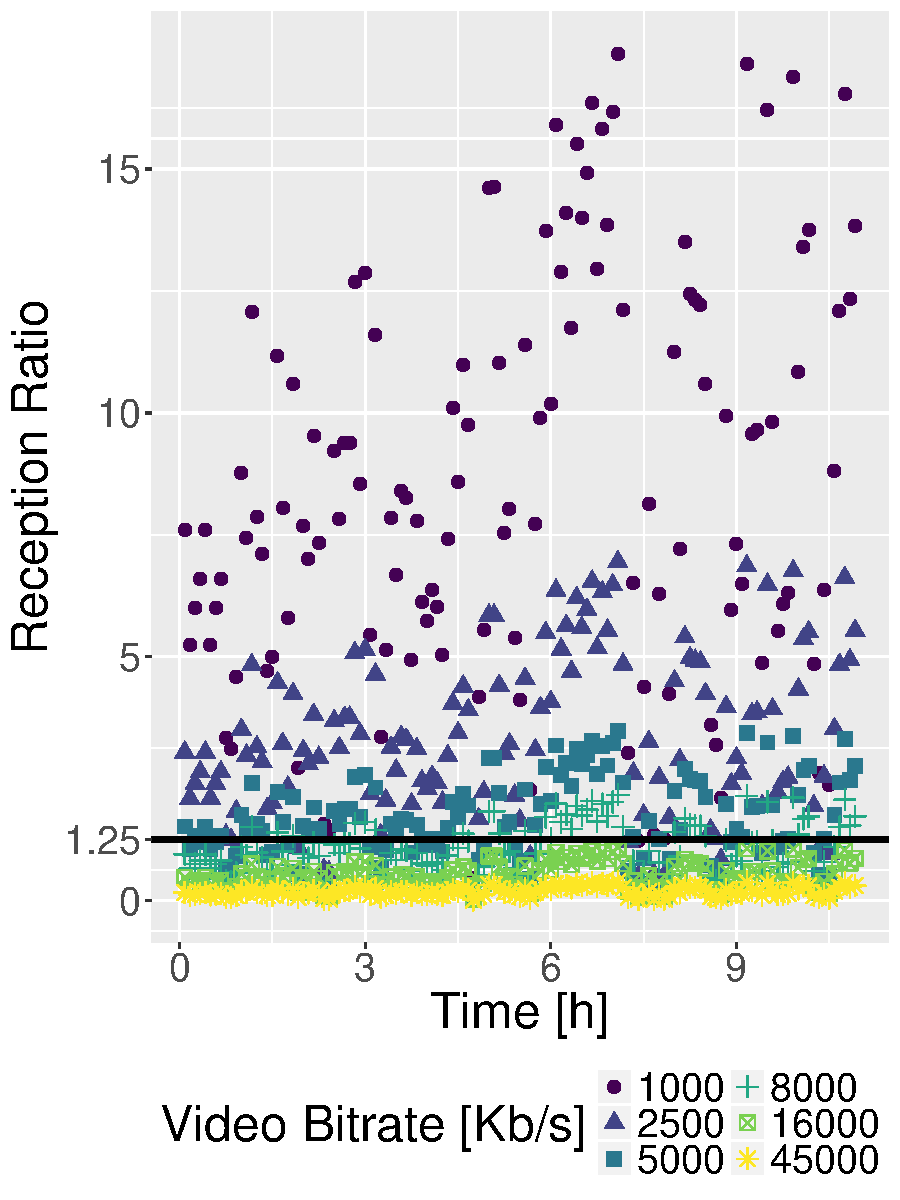
\includegraphics[width=\textwidth]{images/receptionratio-timeseries.pdf}
        \caption{Reception ratio (according to \cite{Hossfeld2013}) time series.}
        \label{fig:receptionratio}
    \end{subfigure}

    \begin{subfigure}[b]{0.45\columnwidth}
        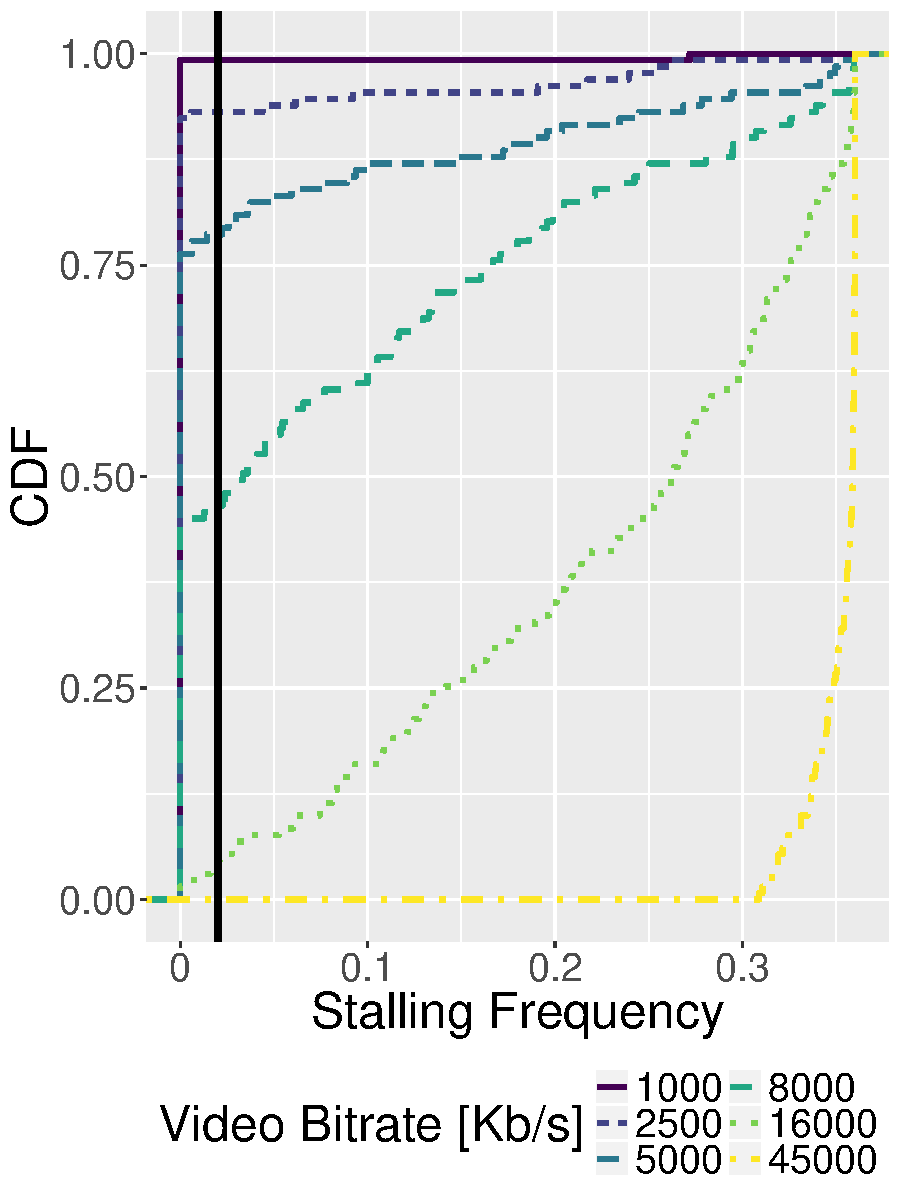
\includegraphics[width=\textwidth]{images/stallingfreq-cdf.pdf}
        \caption{Corresponding CDF of the stalling frequency.}
        \label{fig:stallingfreq-cdf}
    \end{subfigure}
    ~
    \begin{subfigure}[b]{0.45\columnwidth}
        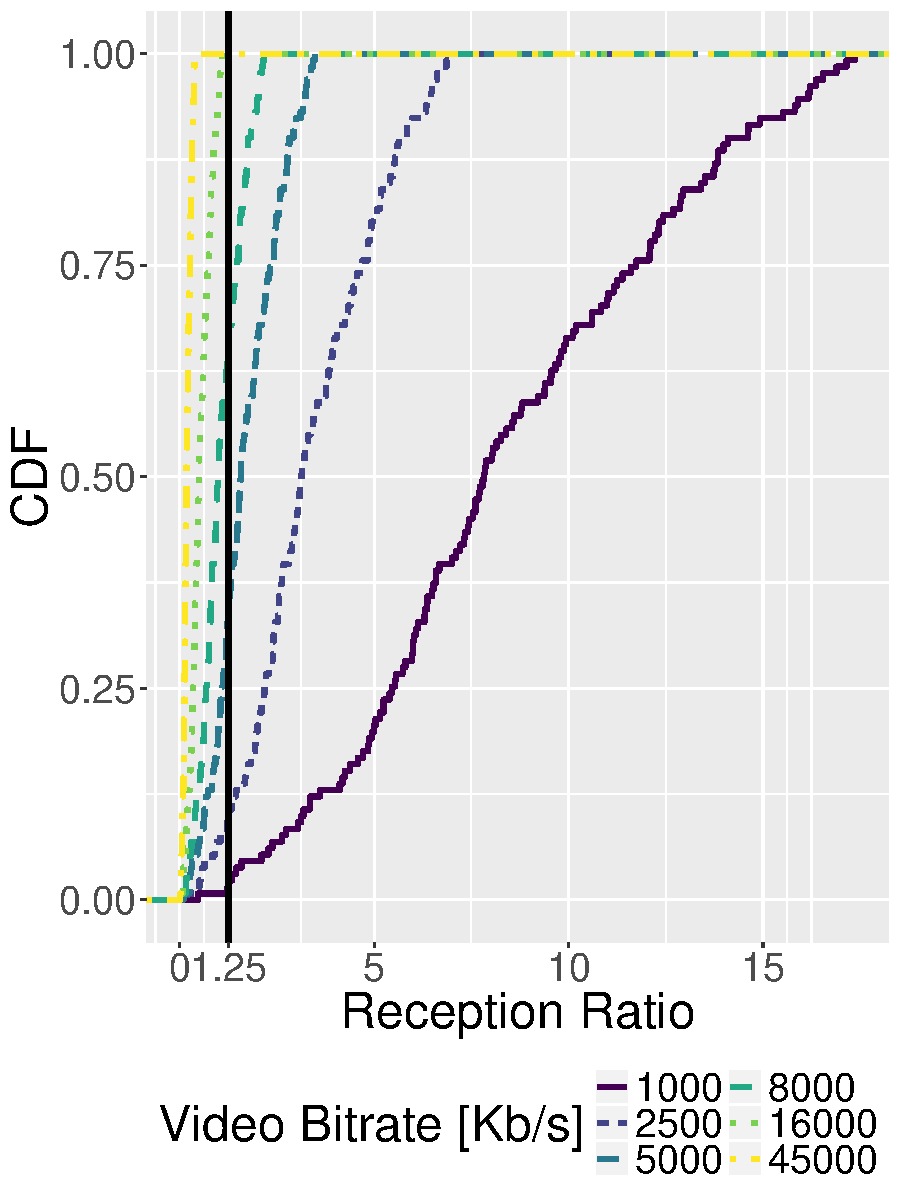
\includegraphics[width=\textwidth]{images/receptionratio-cdf.pdf}
        \caption{Corresponding CDF of the reception ratio.}
        \label{fig:receptionratio-cdf}
    \end{subfigure}
    \caption{Time series and \acrshort{CDF} depictions of the two derived video streaming quality metrics, matching the throughput to the desired video video bitrate. Horizontal --- respectively vertical --- lines denote the selected cutoff threshold for an acceptable streaming quality.}
    \label{fig:timeseries}
\end{figure}

Each spatial region now has to have a series of bandwidth samples attached to it, taken at different points of time. Figure~\ref{fig:timeseries} demonstrates such a time series for one location as both the stalling frequency and the reception rate with the discussed threshold of $1.25$. This also clearly demonstrates large temporal fluctuations for the playable video quality, which should also be exposed in the community quality map, e.g. through some additional, advanced information overlays for each location. Yet, the default geographical map should be kept free of such temporal data to avoid overwhelming the users.

In order to provide a clutter-free representation the mapping service needs to decide for just one specific video quality rating at each location. This requires some form of temporal averaging to be conducted. Here, the system will color the map in the highest video quality of which \SI{90}{\percent} of the bandwidth samples over the measured period were above $1.25 \times V$.

Both the more complex stalling frequency --- using a similar threshold of \SI{2}{\percent} here --- and the reception ratio representation result in the same quality decisions here. Moreover, the two metrics have a Pearson correlation coefficient of $-0.92$. This means that even this simple metric is sufficiently able to visualize the service's quality, and no more complex metric needs to be employed here. With this, the results also become easily comparable to other approaches  (e.g. YouSlow\cite{Nam:2014:YPA:2619239.2631433}) that rely on directly measuring the rebuffering rate (which is akin to the stalling frequency $F$). A mockup of the resulting geographical map and video quality overlay is shown in Figure~\ref{fig:videoquality-map}. Common caveats of geographical grouping and interpolation of samples also apply to this type of video quality map and still need to be solved.

\begin{figure}[!t]
	\centering
	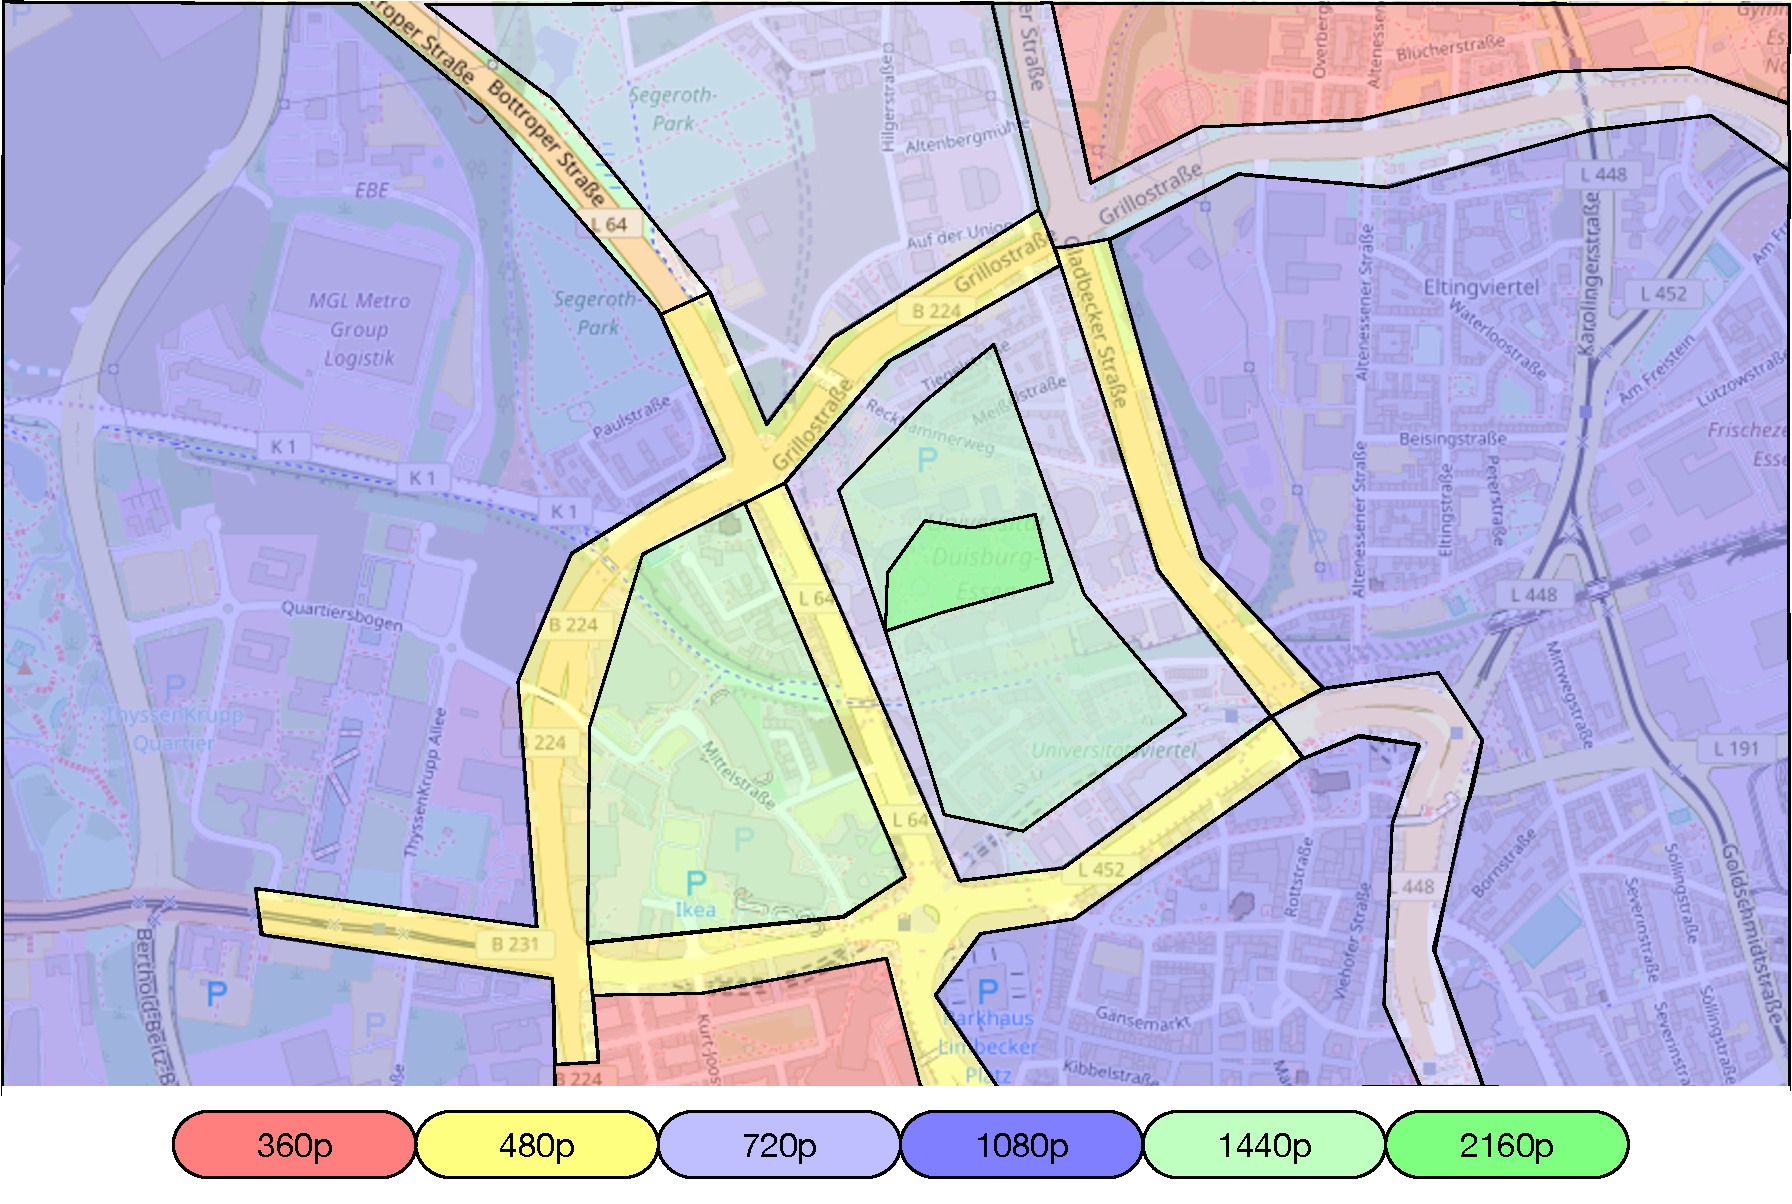
\includegraphics[width=1.0\columnwidth]{images/qoe-map-mockup.pdf}
	\caption{Mockup map of achievable YouTube video resolution for specific regions for a mobile provider. Regions should be grouped and interpolated from individual participants' measurements.}
\label{fig:videoquality-map}
\end{figure}


Now consider this map for a hypothetical use case of someone having to move to a new place. It is common today to check the new apartment's location for good internet access, both wired as well as mobile. Using our approach that person would then not just be able to tell if there is connectivity in that area --- as in most other participatory sensing approaches --- but also if a specific service works in an acceptable quality there, especially at the time of day when one is at home.

While YouTube does serve as the example here, it is important to note that, with the available throughput data, similar mappings and visualizations can easily be achieved for any other kind of service. This is just a matter of switching the mapping function to another, appropriate one for that service. This would allow the community crowdsensed map to be easily extensible and able to be personalized to show the quality of one's favorite services. All while still avoiding to collect resource-intense service-specific data and therefore able to easily scaled up to a large community.


% \begin{table}
% \caption{Confusion matrix of ratio of $F$ and $\rho$ values above and below the associated thresholds of $0.02$ for $F$ and $1.25$ for $\rho$.}
% \label{tab:confused}
% 	\begin{tabu}{XXX}
% 		\toprule
% 		 & \textbf{Better or equal than threshold} & \textbf{Worse than threshold} \\
% 		 \midrule
% 		$\mathbf{F}$ & \SI{53.7}{\percent} & \SI{46.3}{\percent} \\
% 		$\boldsymbol{\rho}$ & \SI{48.2}{\percent} & \SI{51.8}{\percent} \\
% 		\bottomrule
% 	\end{tabu}
% \end{table}



% This can now be combined with the geographical location, the time of measurement, and radio information attached to the throughput sample. From this the video resolution that is playable without downscaling or stalling at the recorded location is calculated and similar results can now be grouped together to be presented on a geographical map. Grouping spatial samples comes with a set of issues of its own, especially when considering temporal variations that are commonplace in radio networks. For this prototype, we envisioned a simplistic approach like taking the convex hull of the same video quality ratings, other grouping approaches and a better spatial analysis are being considered for the future. Figure~\ref{fig:videoquality-map} depicts a mockup of such a video resolution map.


%, and approaches which make available only this data to the public might not be directly helpful or even misleading.


%Mention the usual geodesic and spatial issues of affixing values of certain locations (including temporal variations), especially for radio propagation; take the easy way out and suggest convex hull around similar bandwidth values to group them

%Spatial analysis
%Other spatial grouping and clustering approaches, i.e. detect streets and other ``hot'' areas where a number of data points are grouped closely together


%How to read the map in Figure~\ref{fig:videoquality-map}: In each colored region, users in the specified mobile network are expected to be able to watch YouTube videos with their devices in the specified quality without any (or very few) stalling events or downward quality adjustments during \gls{HAS} operation.

%I.e., the actual community benefits from our approach.



%!TEX root = paper.tex
%%%%%%%%%%%%%%%%%%%%%%%%%%%%%%%%%%%%%%%%%%%%%%%%%%%%%%%%%%%%%%%%%%%%%%%%%%%%%%%%
\section{Conclusion}
\label{sec:conclusion}

The approach taken here attempts to combine the strengths of participatory crowdsensing with the knowledge garnered by the \gls{QoE} community in recent years in order to provide the public with a type of information --- the attainable YouTube video quality at a specific location in a mobile network--- that has much more immediate utility than providing simple measured network \gls{QoS} samples. Such a large-scale crowdsensing endeavor can only be achieved through some compromises as they have been taken here. Actively conducting subjective video \gls{QoE} user studies at each location is equally unfeasible as is being wasteful with the participants' devices' resources, especially with stringent bandwidth data caps in place.

All in all, we think that our approach of conducting large scale low-volume bandwidth estimation measurements and transforming them through adequate \gls{QoE} mapping might be much more engaging for a wider audience and thus indicative of the future to come.

\section*{Acknowledgments}
We would like to thank Michael Jokic for his contributions. The work on bandwidth estimation is based on his 2016 master's thesis ``Analyse von Bandbreitenmessmethoden in mobilen Netzen'' \cite{jokic16mobileBW}.

\balance
\printbibliography

\end{document}
